\chapter{Design}
\label{cha:design}

As detailed in the previous chapters, the Spoofax Language Workbench already
offers a wide variety of services to assist in developing new domain specific
languages. However, not all exposed functionality can be used easily from within
the context of a REPL, where a user wants to be able to type in some expressions
and see their results.

An example is the various transformation goals made available to the user by a
language designer. There is no such thing as a uniform ``evaluation command''
that works across all languages. Instead, each language defines its own
transform goals, of which one is an evaluation goal.  Furthermore, the sequence
of processing steps needed to go from source to parsed source to a transformed
result also varies between languages. One of the main goals that the design had to
accomplish therefore, was to expose a uniform interface for the various
transformation stages to REPL frontends.

In \cref{sec:overview} an overview of the product design and its various
components is given first. Afterwards, the individual components are
explained in more depth. In \cref{sec:commands} the presentation of a uniform
interface to frontends by encapsulating operations in commands is addressed.
\Cref{sec:function-comp} details how commands have been
decomposed into smaller functions, which allows frontend to build their own
transformation pipeline. \Cref{sec:visitor} then explains how this
transformation result is returned to the REPL frontends.

Finally, in \cref{sec:eval-strat}, the DynSem evaluation strategy is outlined. 
An explanation is given as to how other evaluation strategies
can be added to the existing design to support other interpreter backends,
such as Stratego.

\section{Overview}
\label{sec:overview}

As stated in \cref{ssec:goals}, one of the design goals during the project was
to keep the implementation of the REPL IDE-agnostic. To achieve this goal, the
product has been split into a backend and several frontends. This backend
interacts with the Spoofax services on behalf of the frontends. An overview of
its design can be found in \cref{fig:uml-overview}. To request and receive
results from the backend, every frontend should at least implement the
\texttt{IResultVisitor} interface in the \texttt{client} package and
acquire an instance of a class implementing the \texttt{ICommandInvoker}
interface.

The \texttt{ICommandInvoker} instance maintains a map from command names to
corresponding \texttt{IReplCommand} instances. A frontend can thus send
input directly to the \texttt{execute} method, after which the command
corresponding to the input is resolved and executed. The executed command
then returns an instance of a class implementing the \texttt{IResult}
interface. The actual type of the returned class depends on the executed command
and whether the command was successful or not. The frontend is itself
responsible for deciding how to present the result types to the user.

\begin{figure}[h!]
  \centering
  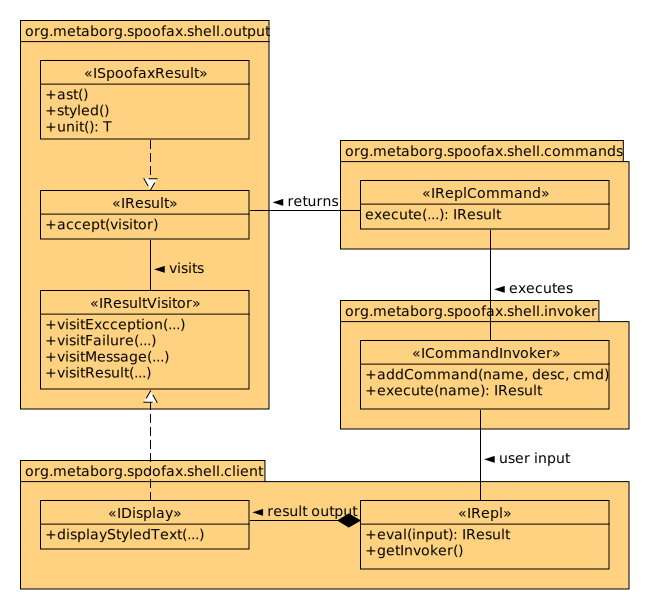
\includegraphics[width=0.75\textwidth]{uml-overview}
  \caption{An overview of the most relevant components of the backend.}
  \label{fig:uml-overview}
\end{figure}


\section{REPL Commands}
\label{sec:commands}

To separate the implementation of user operations into logical units, each user
operation is encapsulated within a class implementing the
\texttt{``IReplCommand''} interface. See \cref{fig:uml-commands} for the design
of the \texttt{commands} package. After acquiring an invoker instance, the
frontend has two commands available by default:

\begin{description}
  \item [:load] \texttt{LanguageCommand}, loads a language from a file path;
  \item [:help] \texttt{HelpCommand}, prints descriptions of all available commands.
\end{description}

\begin{figure}[h]
  \centering
  \includegraphics[width=\textwidth]{uml-commands}
  \caption{UML of the various commands frontends can execute and the
           corresponding result interfaces.}
  \label{fig:uml-commands}
\end{figure}

Frontends can define additional commands by implementing the
\texttt{``IReplCommand''} interface. These commands can then be made available
to the invoker by either binding them in the default map of available commands
via a Guice module or by adding an entry to the invoker at runtime using the
\texttt{``addCommand''} method.

As explained in the introduction of this chapter, there are only a few
commands that work across all languages, since every language can define its
own transformations or evaluation strategy. Therefore, the
\texttt{LanguageCommand} tries to determine several properties of the loaded
language and adjusts the set of loaded commands accordingly.

By splitting operations in small logical units the design ensures command
classes adhere to the Single Responsibility principle, which makes all REPL
commands less complex and therefore easier to maintain. The logical units that
make up the commands also ensure a flexible design that can be modified
as the Spoofax architecture develops further on.

% FIXME: Belongs in implementation chapter probably.
%The ``LanguageCommand'' tries to load a language using the Spoofax services.
%When Spoofax succeeds in loading the language, the parameters set in the
%language facets (specifically the AnalysisFacet and the ShellFacet) are used to
%create a set of commands that should be available for this specific language
%through the ``CommandBuilder'' class. The resulting set of commands consists of
%the following commands:
%
%\begin{description}
%  \item [:parse] Parses the given arguments and returns a corresponding AST.
%  \item [:analyze] Performs static analysis on the input. Not available in all languages.
%  \item [:evaluate] Evaluates the given input and returns the execution result.
%\end{description}
%
%Furthermore a command is created for each transform goal specified through the
%Spoofax MenuService. The transform commands are identified by their name as
%specified in ESV. The process of building commands will be explained in more
%depth in \cref{sec:function-comp}. By making all these commands

%%% Local Variables:
%%% TeX-master: "../main"
%%% End:


\section{}
\label{sec:function-comp}

\begin{figure}[h]
  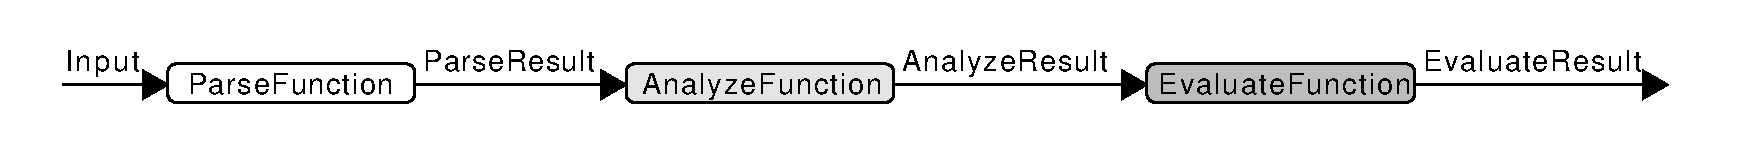
\includegraphics[width=\textwidth]{unit-flow}
  \caption{Processing steps for a language.}
  \label{fig:unit-flow}
\end{figure}


\section{}
\label{sec:visitor}

\section{Evaluation Strategies}
\label{sec:eval-strat}
As explained in \cref{ssec:supp-diff-ways}, there are multiple ways for
specifying the dynamic semantics of a language. Interpretation can for example
be performed through an interpreter generated from a DynSem specification, or by
implementing the interpreter in Stratego or Java. However, ultimately all of
these methods do the same thing. That is, they accept an AST as input and
somehow transform it into an output. In Spoofax, both the AST input and the
output value can be represented as a Stratego term. This is due to the fact that
the format for terms in Spoofax supports all of the basic types that Java has:
integers, real numbers, strings, lists and named constructor applications for
encoding objects~\cite{Brand00}. It is only the internal representation of an
interpreter's evaluation context and the implementation of the interpreter that
differs.

The strategy pattern is a pattern for encapsulating computation tasks that have
the same types of input and output, but a different implementation. This is
precisely the case for the different methods of evaluation: the method or
``strategy'' of evaluation is therefore put behind an interface called
\texttt{IEvaluationStrategy}. \Cref{fig:uml-eval-strat} shows a UML diagram
of this part of the design.

\begin{figure}[t]
  \centering
  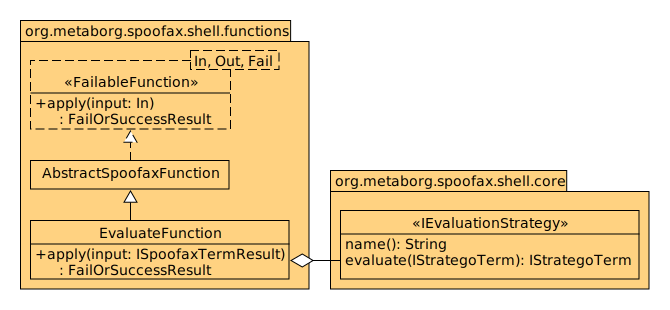
\includegraphics[width=\textwidth]{uml-eval-strat}
  \caption{UML of the \texttt{IEvaluationStrategy} interface and its
    collaborators.}
  \label{fig:uml-eval-strat}
\end{figure}

An implementer of the \texttt{IEvaluationStrategy} is responsible for performing
evaluation on an AST representation of a program within the evaluation context
that it maintains throughout successive invocations. In this way, maintaining
the evaluation context is encapsulated, and no assumptions are made of what the
evaluation context looks like. This is a desirable property since the
representation of an evaluation context varies across languages and evaluation
methods.

%%% Local Variables:
%%% mode: latex
%%% TeX-master: "../main"
%%% End:


%%% Local Variables:
%%% mode: latex
%%% TeX-master: "main"
%%% End:
